Für die Messungen wurden im Laufe des Projekts zwei Versionen an Prototyp-Platinen entworfen. Im Verlauf der Versuche wurden Veränderungen an den Platinen vorgenommen, um den Betrieb dieser zu verbessern. 
\section{Prototyp 1}
%\begin{center}
%\begin{minipage}{0.5\textwidth}
%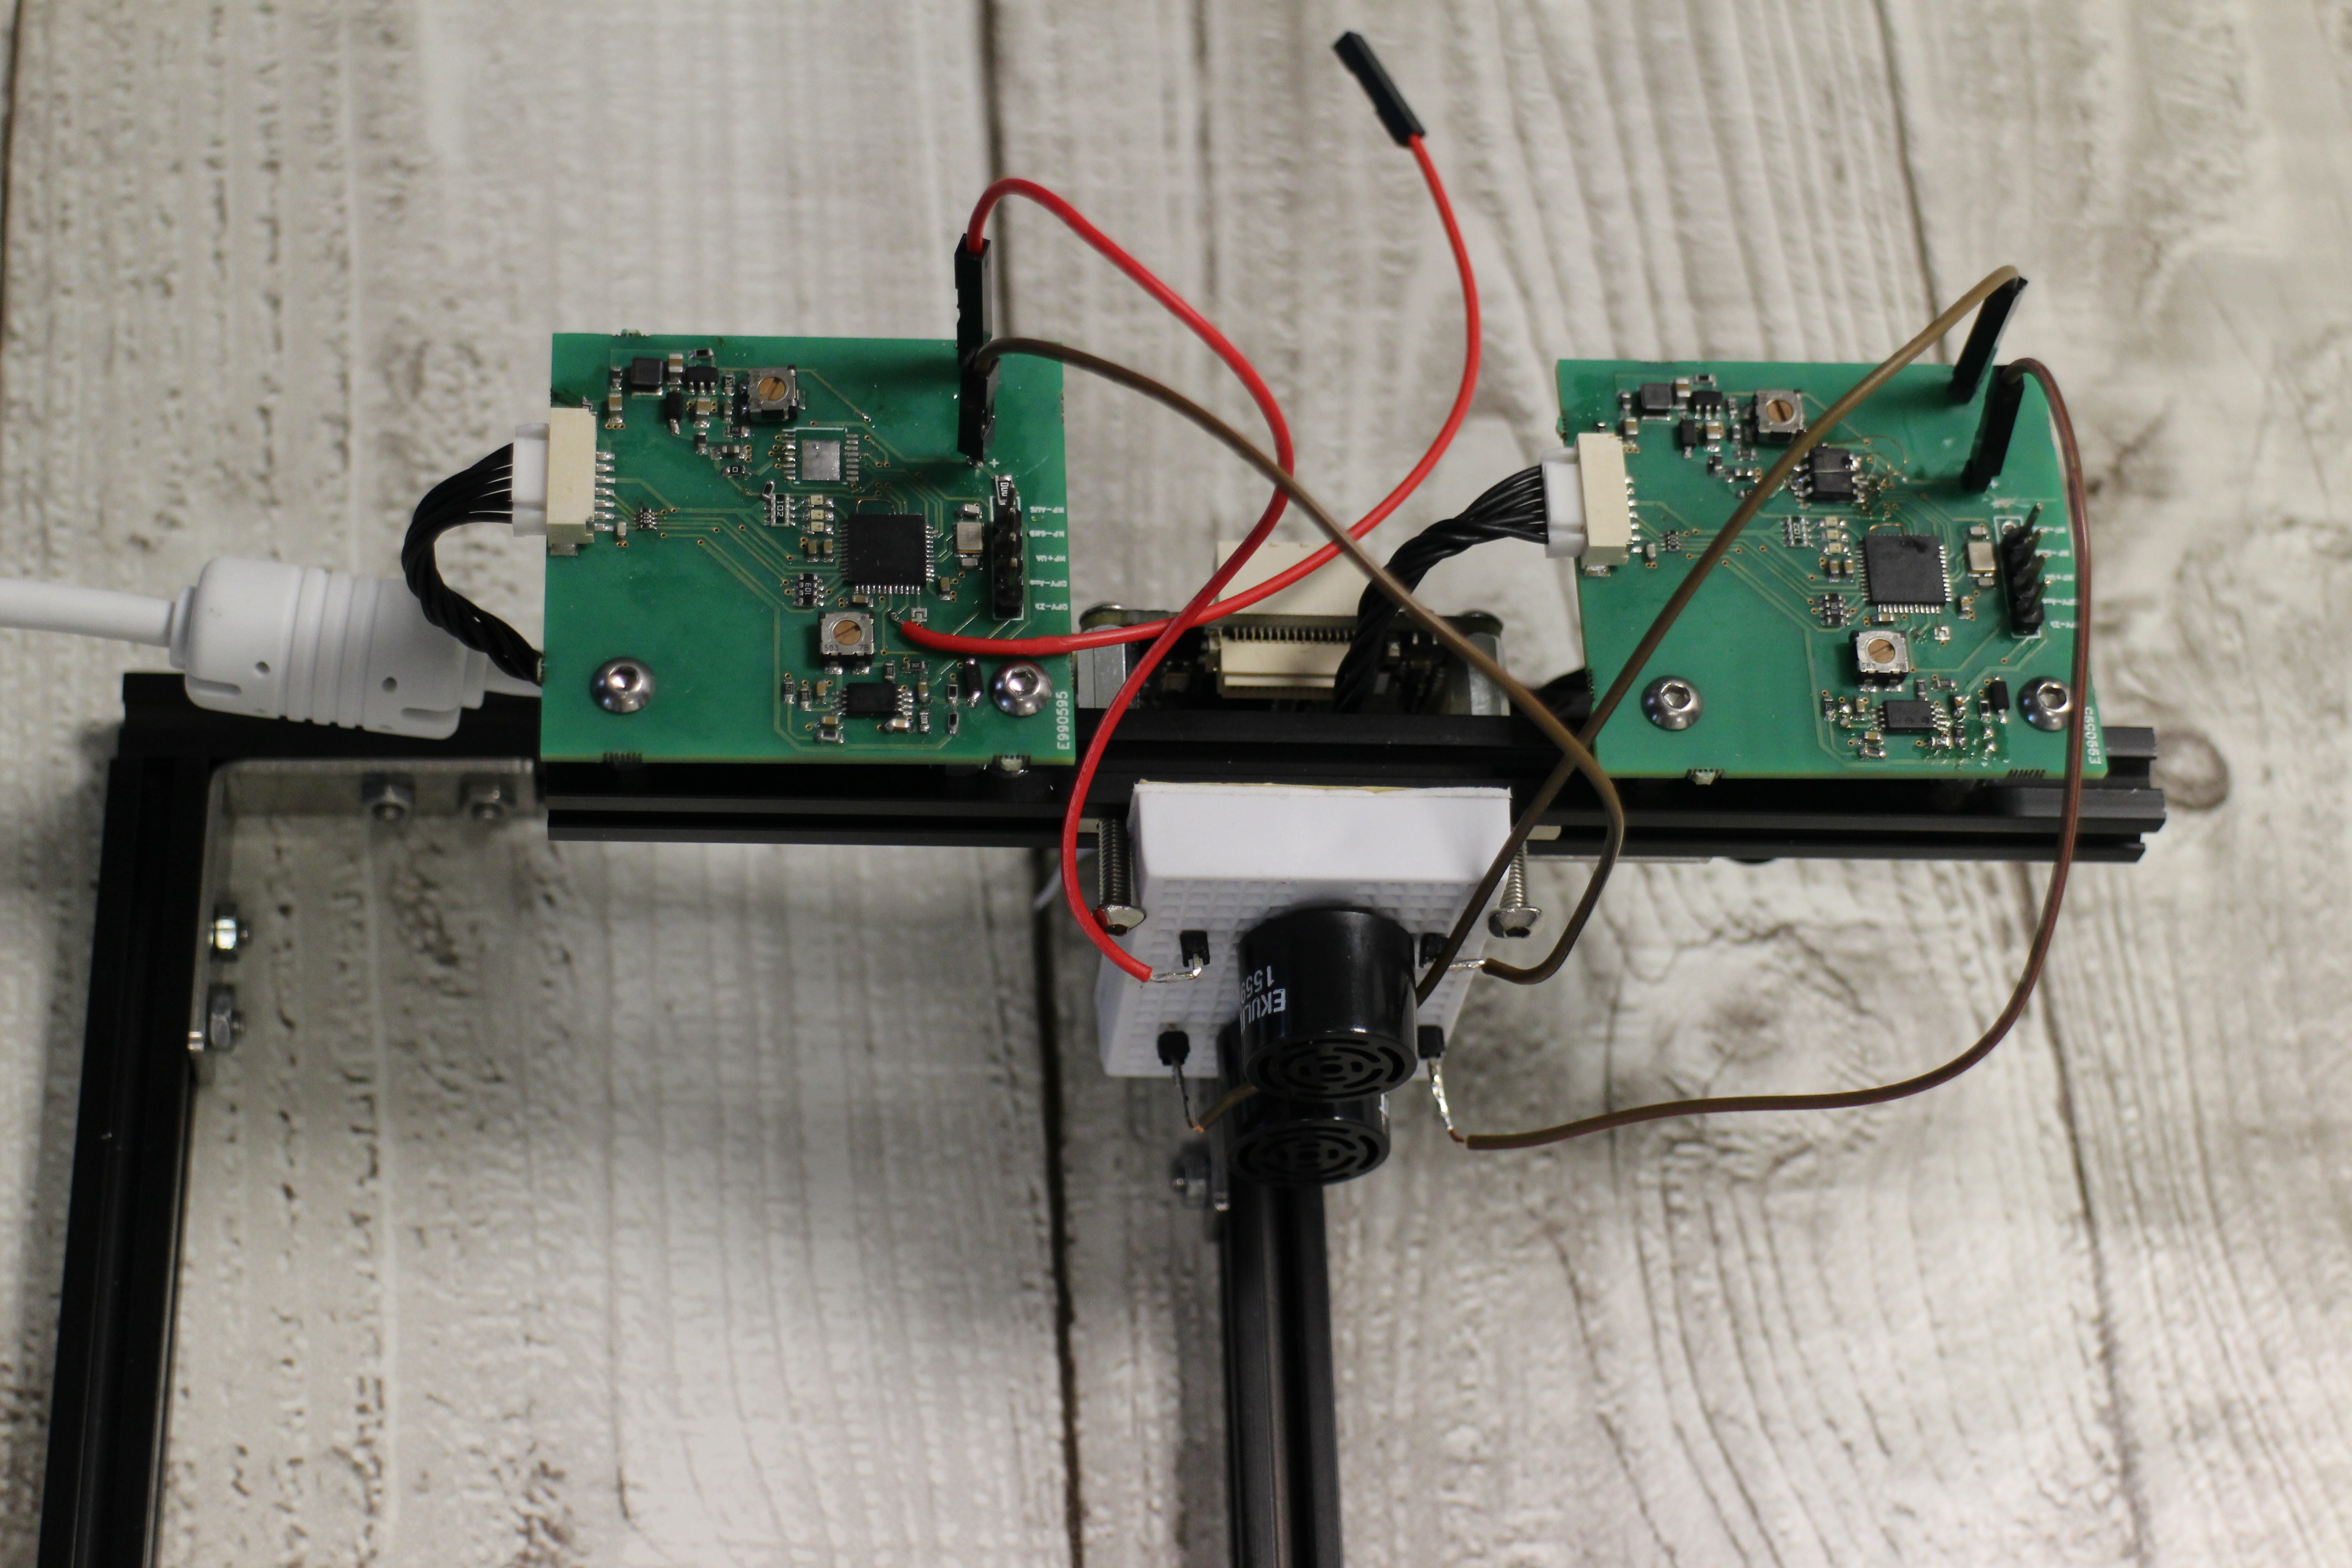
\includegraphics[width=1\textwidth%, draft
%]{Abbildungen/Prototyp1.png}
%\captionof{figure}{Aufebaute und bearbeitete Platine des ersten Prototypen}
%\label{fig:Prototyp1}
%\end{minipage}
%\end{center}
Bei dem ersten Prototyp wurden die Sendereinheit und die Empfängereinheit auf getrennten Platinen aufgebaut. So bestand die Möglichkeit, den Senderkreis und den Empfängerkreis getrennt zu untersuchen, ohne dass sich elektrische Signale der beiden Schaltkreise überlagern konnten. Anfangs wurde für den Senderkreis eine komplette H-Brücke als Schalter verwendet. Allerdings war der Aufbau nicht funktional, da ein Beschaltungsfehler vorhanden war. Dieser wurde mit Fädeldraht provisorisch behoben.  Dadurch, dass das A5950 eine H-Brücke mit integrierter Kontroll-Logik und eigener Spannungspumpe ist, wurde anhand der Schaltweise der Baugruppe festgestellt, dass diese H-Brücke nicht für die Schaltung einsetzbar ist. Um nicht sofort eine neue Platine in Auftrag geben zu müssen, was einiges an Zeit gekostet hätte, wurde das IC einfach ausgelötet. Danach wurde zunächst ein MOSFET als HIGH-Side an der Stelle eingesetzt.Dadurch ließen sich erste Versuche durchführen, allerdings entsprach das Ergebnis noch nicht den Anforderungen. Deswegen wurde die Beschaltung an dieser Stelle auf eine Halbbrücke erweitert. Damit war die Funktion des Senderkreises für die ersten Versuche und Messungen gegeben.\\
Der Empfängerkreis war von Beginn an funktional, konnte aber erst mit Inbetriebnahme des Senderkreises richtig getestet werden. Am Empfängerkreis wurden lediglich zu Testzwecken Änderungen an der Filterung, vor dem Verstärker, vorgenommen. Die Filterung wurde in ihrer Dimensionierung verändert, um herauszufinden, wie sich die Qualität des Echo-Signals verbessern lässt.\\

\subsection{Senderkreis}
Zu erst wurden Signale direkt an der CPU gemessen, um sicher zu stellen, dass die Einstellungen im Programm auch die gewünschten Ausgaben zur Folge haben, und keine Gefärdung der Bauteile entsteht.
Um das Signal für die Entfernungsmessung zu generieren wurde der Mikrocontroller so programmiert, dass zehn Impulse mit einer Frequenz von 40~kHz ausgegeben werden. Danach erfolgt eine Pause, um das zurückkehrende Signal abzuwarten und auszuwerten.\\
\begin{minipage}{0.5\textwidth}
\includegraphics[width=1\textwidth%, draft
]{Abbildungen/MessungenP1/PWM-von-der-cpu.png}
\captionof{figure}{PWM-Burst auf 40~kHz Basis an der CPU}
\label{fig:pwm-burst}
\end{minipage}
\begin{minipage}{0.5\textwidth}
\includegraphics[width=1\textwidth%, draft
]{Abbildungen/MessungenP1/PWM-ausgabe-mit-Hi-Side.png}
\captionof{figure}{PWM Ausgabe über einen HIGH-Side}
\label{fig:HiSide}
\end{minipage}
In der Abbildung \ref{fig:pwm-burst} ist zu sehen, dass der gewünschte Burst aus zehn Impulsen mit einer Periodendauer von jeweils 25~\textmu s vom Mikrocontroller generiert wurde. Diese Messung wurde auch vorgenommen, um zu überprüfen, wie sich das Signal durch die eingesetzten Bauteile verändert.\\
Die Abbildung \ref{fig:HiSide} zeigt, wie das Ausgangssignal nach einer HIGH-Side aussieht. So wird zwar im Takt des PWM-Signals geschaltet, allerdings fehlt es an einem Gegenpol, um das Potential in den Schaltpausen wieder auf Null zu ziehen. Dadurch bleibt die Spannung während des Schaltens immer auf einem erhöhten Pegel und sinkt erst nach Ende des PWM-Signals langsam ab. Dadurch kann natürlich keine vernünftige Ausgabe am Lautsprecher erzeugt werden, denn ohne deutliche Potentialunterschiede kann dieser auch nicht in Schwingungen versetzt werden. Der ausgegebene Schalldruck würde nur für kurze Entfernungsmessungen reichen. Das zurückkommende Signal wird von der abklingenden Spannung des HIGH-Side überlagert. Somit ist dieser Aufbau nicht operabel.\\
Um die Spannung nicht nur auf einen HIGH-Pegel, sondern auch auf einen LOW-Pegel schalten zu können wurde danach auf eine Halbbrücke gewechselt. Mit dieser lässt sich der Ausgang, über zwei durch das PWM-Signal gesteuerte MOSFETs, sauber auf HIGH- oder LOW-Pegel schalten. %Bei der ersten, einfach gesteuerten Version, entstand das Problem, dass beim Schalten der Halbbrücke, beide MOSFETs gleichzeitig geschaltet haben. Dieses klingt zwar nicht nach einem Problem, doch wird es durch die technischen Gegebenheiten zu einem, denn bei den meisten elektronischen Schaltern verläuft der Einschaltprozess deutlich schneller, als der Ausschaltprozess. Wenn also zwei Bauteile gleichzeitig schalten, hat das einschaltende Bauteil schneller eingeschaltet, als das ausschaltende Bauteil ausgeschaltet. Dadurch entstehen bei jedem Schaltvorgang Kurzschlüsse. Auch wenn diese nur für Nanosekunden bestehen, bevor sie wieder unterbrochen werden, ist davon auszugehen, dass zu den dadurch entstehenden Störungen auch Bauteile zerstört werden.\\ Somit wurde auf eine voll gesteuerte Halbbrücke gewechselt und es wurden zwei PWM-Signale moduliert, bei denen eines invertiert und die Flanken derart verschoben waren, dass die angesteuerten MOSFETs nie Kurzschlüsse schalten können.
Mit der verwendeten Halbbrücke ergab sich die Abbildung \ref{fig:Halfbridge}\\
\begin{minipage}{0.5\textwidth}
\includegraphics[width=1\textwidth%, draft
]{Abbildungen/MessungenP1/PWM-Nach-der-Halbbrucke.png}
\captionof{figure}{PWM Ausgabe über eine Halbbrucke}
\label{fig:Halfbridge}
\end{minipage}
\begin{minipage}{0.5\textwidth}
\includegraphics[width=1\textwidth%, draft
]{Abbildungen/MessungenP1/PWM-Nach-der-Halbbrucke-mit-LS.png}
\captionof{figure}{Ausgabe der PWM an der Ultraschallkapsel}
\label{fig:Senderausgabe}
\end{minipage}
Es zeigt sich, dass das Signal nach der Erweiterung auf eine Halbbrücke wieder wie das von der CPU ausgegebene PWM-Signal \ref{fig:pwm-burst} aussieht. Die Amplitude fällt wie geplant höher aus. Somit kann die Höhe der Amplitude über die Spannungspumpe variiert werden um die Stärke des ausgegebenen Signals zu verändern, ohne die CPU durch die höhere Spannung zu beschädigen. Wie in der Abbildung \ref{fig:Senderausgabe} zu entnehmen ist, entstehen durch die angeschlossene Ultraschallkapsel höhere Spannungsimpulse in den Schaltmomenten. Diese Spannungsspitzen, die durch die Ultraschallkapsel entstehen, wurden in den Versuchen vernachlässigt, da keine Gefährdung anderer Bauteile entstand. Das somit generierte Ausgangssignal entsprach den Anforderungen und musste für die Versuche nicht weiter bearbeitet werden.
\subsection{Empfängerkreis}
Die Platinen des Sender- und Empfängerkreises wurden gemeinsam auf einer Halterung montiert, so dass die Ultraschallkapseln zum senden und empfangen der Signale nebeneinander befestigt werden konnten. Ziel war es, durch verschieben eines Hindernisses die Signaländerungen an den Platinen beobachten zu können, ohne die gesamten Messaufbauten bewegen zu müssen. Bei der Aufnahme der Messungen wurde der Empfängerkreis Schritt für Schritt überprüft um zu erfahren, wie sich das empfangene Signal durch die einzelnen Bauteile verändert.\\
\begin{minipage}{0.5\textwidth}
\includegraphics[width=1\textwidth%, draft
]{Abbildungen/MessungenP1/Signal-Empfang.png}
\captionof{figure}{Signal Empfang}
\label{fig:Empfang am LS}
\end{minipage}
\begin{minipage}{0.5\textwidth}
\includegraphics[width=1\textwidth%, draft
]{Abbildungen/MessungenP1/Signal-nach-Verstarkung.png}
\captionof{figure}{Signal nach Verstärkung}
\label{fig:Verstaerkung}
\end{minipage}
Die Abbildung \ref{fig:Empfang am LS} zeigt das Signal, das direkt am Empfänger zu messen war. Hier sind verschiedene vorerst nicht zuordenbare Signale zu sehen. Allein aus diesem Bild lässt sich daher keine Aussage zu den einzelnen Signalen machen. Fest steht nur, dass ebenfalls Signale die nicht der gewünschten Frequenz entsprechen, vom Empfänger aufgenommen werden. Dies gilt es natürlich schnellst möglich auszumerzen, um unerwünschte Störungen zu vermeiden.
Die Abbildungen \ref{fig:Verstaerkung} und \ref{fig:Verstaerkung2} zeigen den Verlauf des Signals nach der Filterung und Verstärkung in zwei verschiedenen Zeitauflösungen. Dabei entspricht \ref{fig:Verstaerkung} den ersten drei Kästchen von \ref{fig:Verstaerkung2} und dient um darzustellen, dass die Verstärkung eine maximale Aussteuerung von 3,3~V nicht überschreitet.\\
\begin{minipage}{0.5\textwidth}
\includegraphics[width=1\textwidth%, draft
]{Abbildungen/MessungenP1/Signal-nach-Verstarkung2.png}
\captionof{figure}{Signal nach Verstärkung2}
\label{fig:Verstaerkung2}
\end{minipage}
\begin{minipage}{0.5\textwidth}
\includegraphics[width=1\textwidth%, draft
]{Abbildungen/MessungenP1/Signal-nach-Komparator.png}
\captionof{figure}{Signal nach Komparator}
\label{fig:Komparator}
\end{minipage}\\
Nach dem das Signal den Komparator passiert hat, ergibt sich das Bild wie in Abbildung \ref{fig:Komparator} zu sehen ist. Bei einem Vergleich mit dem Signal nach der Verstärkung \ref{fig:Verstaerkung2} wird sichtbar, dass der Komparator nur Signale, die über seinem Schwellwert von 1,8~V liegen, durchschaltet. Die Aufteilung in zwei Signalblöcke in den Abbildungen kommt daher, dass der erste Block das Signal der Sender-Kapsel ist, das direkt beim Senden seitlich auf die Empfänger-Kapsel abgestrahlt wurde. Der zweite Block ist bereits das Echo, das vom 20~cm entfernten Hindernis zurückgeworfen wurde.\\
Anhand dieser Ergebnisse kann festgehalten werden, dass die einfachere Version des Ultraschall-Entfernungsmessers durchaus simpel umzusetzen ist. Es fehlt nur noch ein Programm, das die Zeit zum eintreffen des Echo-Signals in einen Abstand zum Hindernis konvertiert. Besagtes Programm wurde nicht für diese Prototypversion erstellt, da der Anspruch bestand, den Betrieb nicht nur über eine Platine, sondern auch noch über eine Ultraschallkapsel ablaufen zu lassen.
\newpage
\section{Prototyp 2}
%\begin{center}
%\begin{minipage}{0.5\textwidth}
%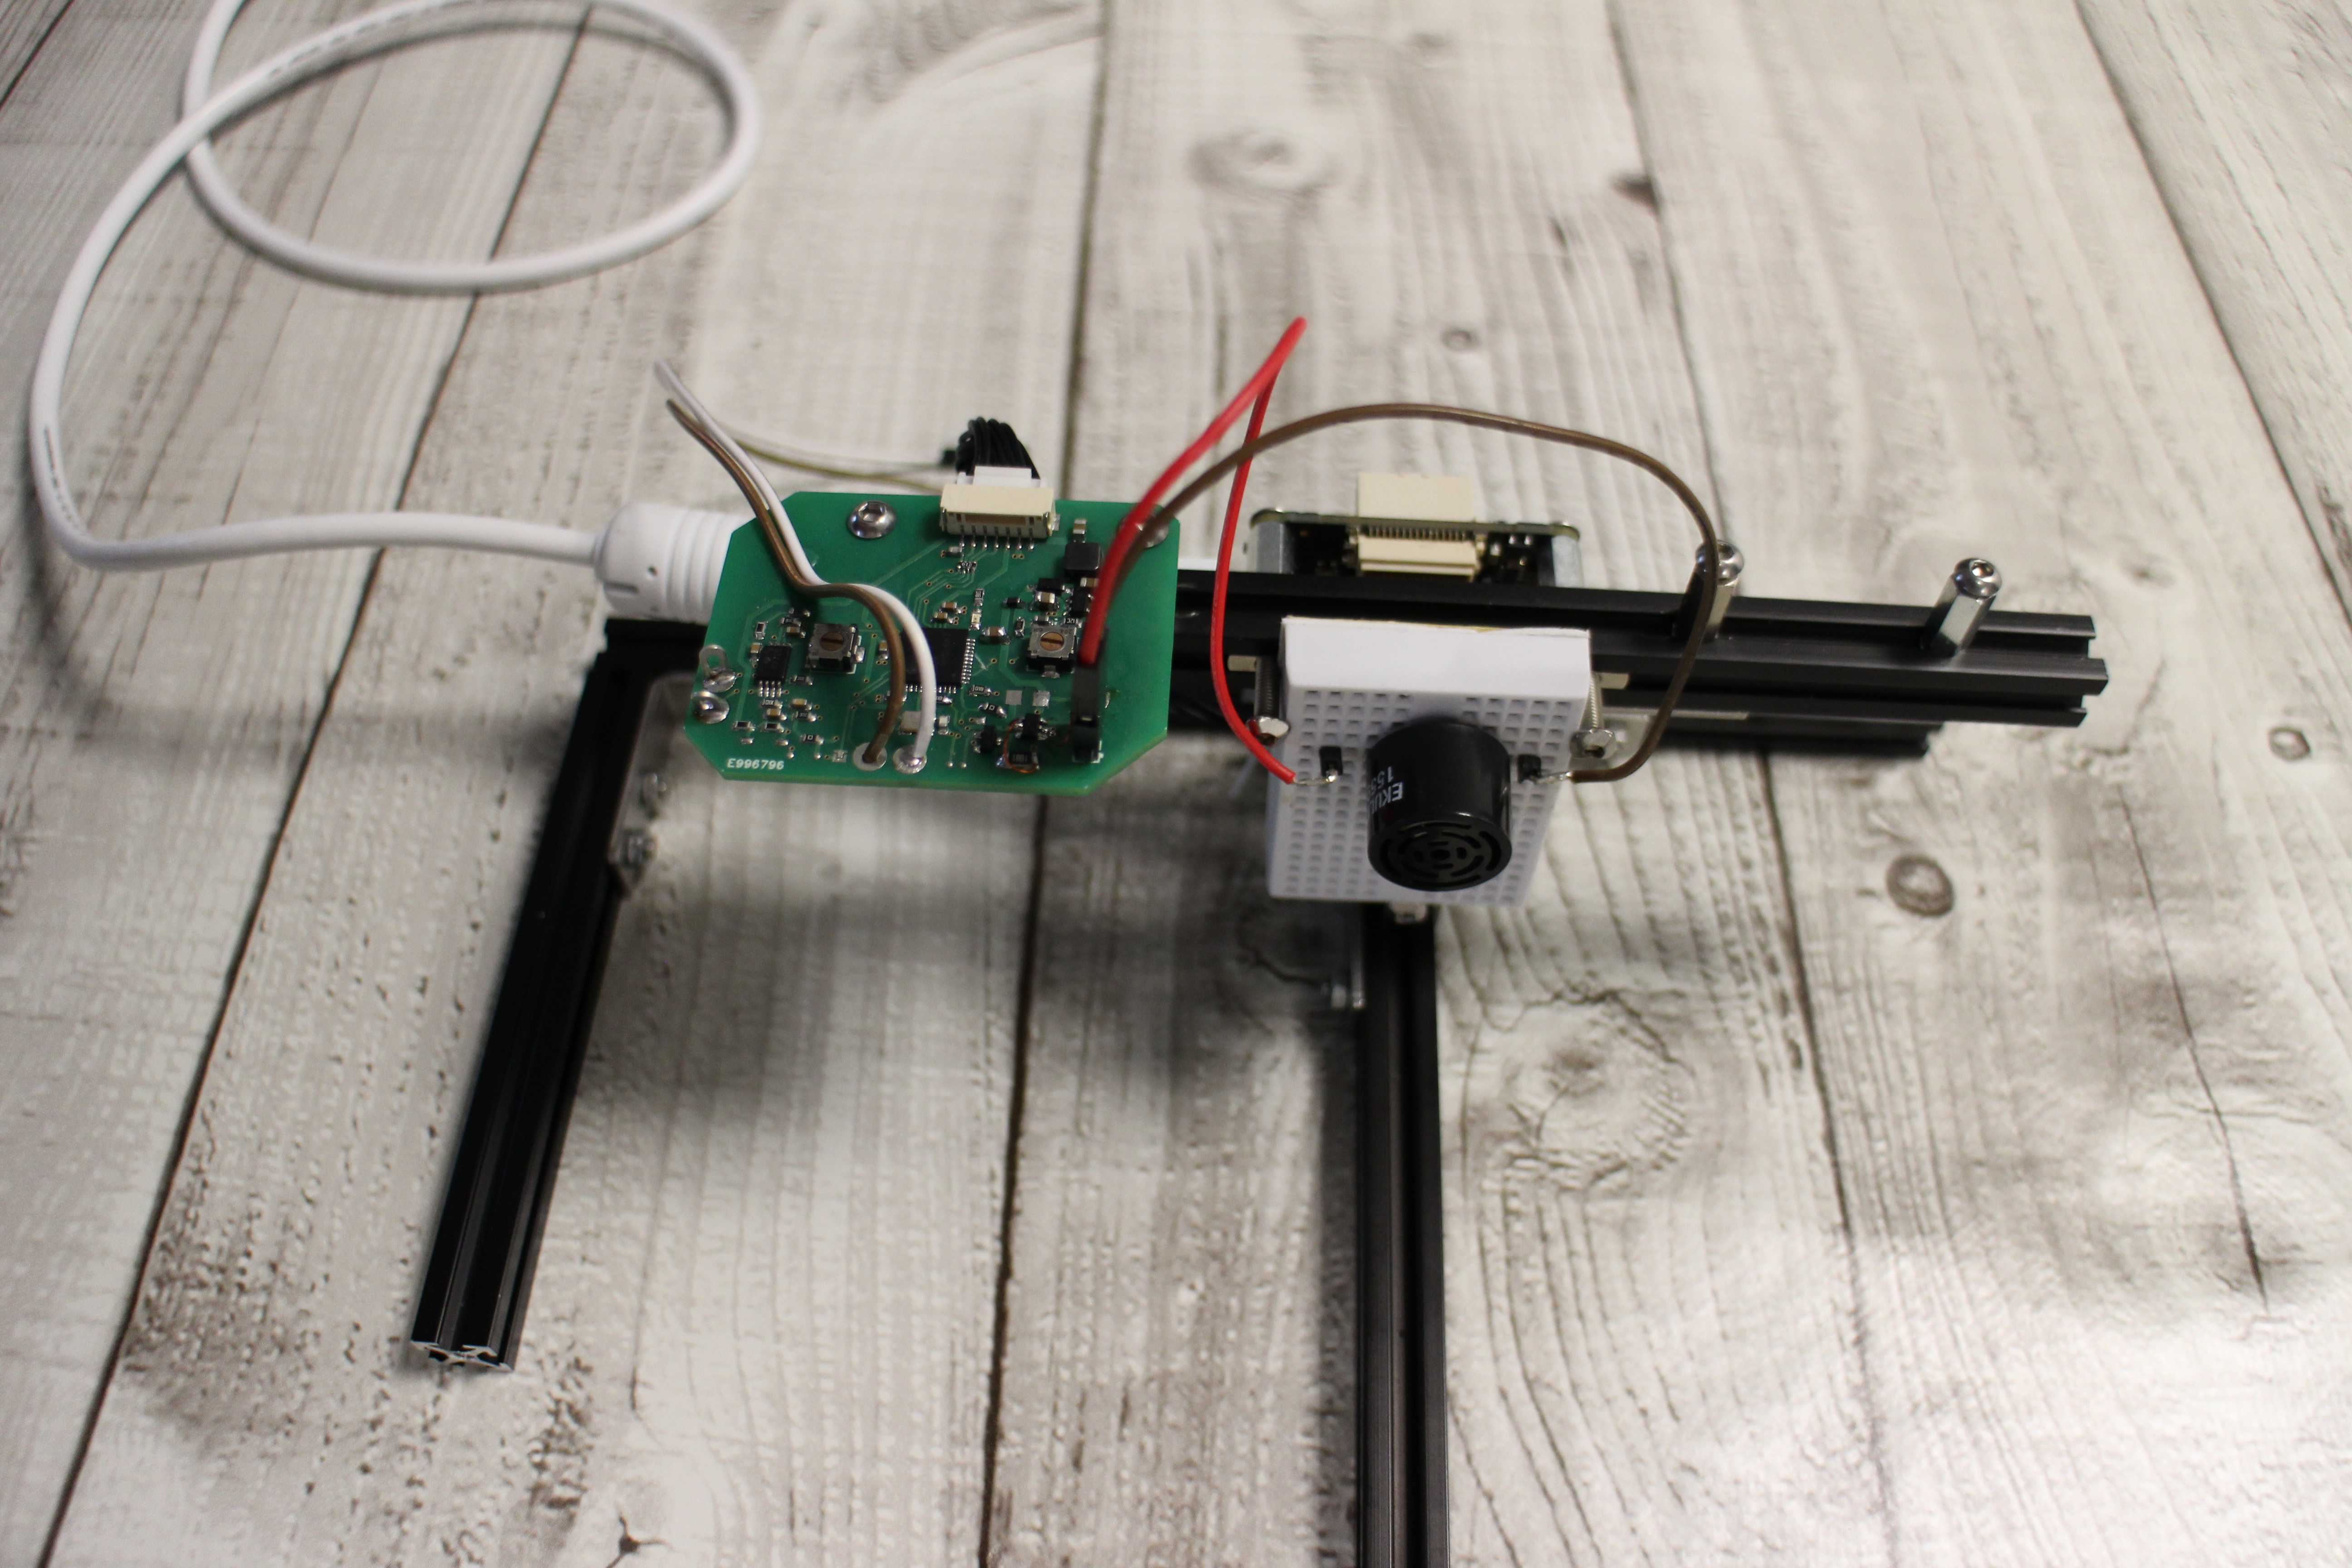
\includegraphics[width=1\textwidth%, draft
%]{Abbildungen/Prototyp2.png}
%\captionof{figure}{Aufebaute und bearbeitete Platine des zweiten Prototypen}
%\label{fig:Prototyp2}
%\end{minipage}
%\end{center}
Nachdem mit der ersten Prototyp-Version bereits Versuche an der Elektronik durchgeführt wurden und auch erste Messungen mit einem beweglichen Hindernis auswertbare Ergebnisse brachten, wurde eine zweite Prototyp-Version entworfen. Bei der zweiten Prototyp-Version wurden der Sender- und der Empfängerkreis auf einer Platine aufgebaut und es wurde nur noch eine Ultraschallkapsel für beide Anwendungen vorgesehen. Dadurch wurden für den fehlerfreien Betrieb drei und nicht zwei Schaltzustände der Halbbrücke benötigt. Deswegen wurde die Halbbrücke der ersten Prototyp-Version durch eine voll gesteuerte Halbbrücke ersetzt. Nicht nur sollte die Ultraschallkapsel mit HIGH-, oder LOW-Signal ansteuerbar sein, auch ein dritter potentialfreier Zustand war nötig, damit die Echo-Signale auch empfangen werden konnten. Um bei diesem Aufbau einen fehlerfreien Betrieb der verwendeten voll gesteuerten Halbbrücke sicherzustellen wurden durch den Mikrocontroller zwei getrennte PWM-Signale generiert die wie in Abbildung \ref{fig:PWMs} zu sehen ist durch Lücken getrennt sind. Verzögerungen im Schaltbetrieb der Halbleiter konnten daher, keine Kurzschlüsse mehr verursachen. Außerdem konnten durch den neuen Platinenentwurf die ab der ersten Prototyp-Version vorgenommenen Änderungen direkt in den Schaltplan übernommen werden. Dadurch ließ sich die Störanfälligkeit durch empfindliche Drahtbrücken deutlich reduzieren. Bedingt durch anfängliche Befürchtungen wurden für die MOSFETs der Halbbrücke anfangs jeweils ein weiteres MOSFET vorgeschaltet. Dieser Zusatz stellte sich als unnötig heraus, da durch eines der zusätzlichen Bauteile eines der PWM-Signale invertiert wurde. Somit wurde das überflüssige MOSFET entfernt. Durch zwei Drahtbrücken konnte die komplette Schaltung nach Entlarvung eines weiteren Verdrahtungsfehlers, in Betrieb genommen werden.\\
\begin{minipage}{0.75\textwidth}
\includegraphics[width=1\textwidth%, draft
]{Abbildungen/MessungenP2/Zwei_PWMs_von_der_CPU.PNG}
\captionof{figure}{Verlauf der zwei generierten PWMs für den Betrieb der voll gesteuerte Halbbrücke}
\label{fig:PWMs}
\end{minipage}\\
Nachdem dieser Betrieb sichergestellt war, wurden Messungen am Verstärker (obere Linie), und am Komparator (untere Linie) vorgenommen. Dabei wurde die Verstärkung so eingestellt, dass unerwünschte Störungen nicht vom Komparator weitergegeben wurden. Die Spannung für den Sendebetrieb wurde für die Versuche zwischen 5V und 20V variiert, um betrachten zu können, wie sich das auf die Reichweite und Genauigkeit der Messungen auswirkt. Als Hindernis wurde bei allen Versuchen eine glatte Holzplatte der Maße 50x64cm verwendet und in einem Abstand von ein bis fünf Metern von der Ultraschallkapsel entfernt aufgestellt. In den Abbildungen \ref{fig:5v1m} bis \ref{fig:5v4m} sind die Ergebnisse einer Messreihe mit einer Spannung von 5~V für den Sendebetrieb dargestellt. Die Ansicht wurde so eingestellt, dass zwei Sendeimpulse zu sehen sind. Dadurch wird deutlicher, welches die Sende Impulse sind, und welches die von der Entfernung abhängigen Echos sind.\\
\begin{minipage}{0.5\textwidth}
\includegraphics[width=1\textwidth%, draft
]{Abbildungen/MessungenP2/5V/1mb.PNG}
\captionof{figure}{Signalverlauf bei 5~V auf 1~m Abstand}
\label{fig:5v1m}
\end{minipage}
\begin{minipage}{0.5\textwidth}
\includegraphics[width=1\textwidth%, draft
]{Abbildungen/MessungenP2/5V/2mb.PNG}
\captionof{figure}{Signalverlauf bei 5~V auf 2~m Abstand}
\label{fig:5v2m}
\end{minipage}
\begin{minipage}{0.5\textwidth}
\includegraphics[width=1\textwidth%, draft
]{Abbildungen/MessungenP2/5V/3mb.PNG}
\captionof{figure}{Signalverlauf bei 5~V auf 3~m Abstand}
\label{fig:5v3m}
\end{minipage}
\begin{minipage}{0.5\textwidth}
\includegraphics[width=1\textwidth%, draft
]{Abbildungen/MessungenP2/5V/4mb.PNG}
\captionof{figure}{Signalverlauf bei 5~V auf 4~m Abstand}
\label{fig:5v4m}
\end{minipage}
Bei den Abbildungen ist zu sehen, dass das Echo-Signal mit zunehmender Entfernung immer schwächer wird. Bei einer Entfernung von vier Metern (Abbildung \ref{fig:5v4m}) wird das Echo-Signal so schwach, dass die Signalstärke nach dem Komparator nicht mehr für eine eindeutige Auswertung über den Mikrocontroller ausreicht. Nachfolgend sind die Abbildungen einer Messreihe mit verschiedenen Spannungseinstellungen für den Sendebetrieb zu sehen. Anhand dieser Messreihe soll dargestellt werden, welchen Einfluss die eingestellte Spannung im Sendebetrieb auf die Reichweite des Ultraschallsignals hat. Für die Darstellung wurden die Messungen bei 5 Meter Abstand ausgewählt.\\
\begin{minipage}{0.5\textwidth}
\includegraphics[width=1\textwidth%, draft
]{Abbildungen/MessungenP2/5V/5m.PNG}
\captionof{figure}{Signalverlauf bei 5~V auf 5~m Abstand}
\label{fig:5v5m2}
\end{minipage}
\begin{minipage}{0.5\textwidth}
\includegraphics[width=1\textwidth%, draft
]{Abbildungen/MessungenP2/10V/5mb.PNG}
\captionof{figure}{Signalverlauf bei 10~V auf 5~m Abstand}
\label{fig:10v5m}
\end{minipage}
\begin{minipage}{0.5\textwidth}
\includegraphics[width=1\textwidth%, draft
]{Abbildungen/MessungenP2/15V/5mb.PNG}
\captionof{figure}{Signalverlauf bei 15~V auf 5~m Abstand}
\label{fig:15v5m}
\end{minipage}
\begin{minipage}{0.5\textwidth}
\includegraphics[width=1\textwidth%, draft
]{Abbildungen/MessungenP2/20V/5mb.PNG}
\captionof{figure}{Signalverlauf bei 20~V auf 5~m Abstand}
\label{fig:20v5m}
\end{minipage}
Bei Vergleich der Abbildungen \ref{fig:5v5m2} und \ref{fig:10v5m} mit den Abbildungen \ref{fig:15v5m} und \ref{fig:20v5m}  ist zu sehen, dass bei einem Abstand von 5 Metern erst bei einer Sendespannung von über 10~V, auch am Komparator ein über den Mikrocontroller auswertbares Signal vorhanden ist. \\
In der nachfolgenden Tabelle \ref{tab:Entfernungsmessung} wurden die Zeitabstände vom ersten Impuls des gesendeten Signals, bis zum ersten Impuls des Echo-Signals aufgetragen. Anhand der Schallgeschwindigkeit die Entfernung, die der Schall zurückgelegt hat berechnet. Dazu wurde noch die Abweichung der berechneten Entfernung von der eingestellten Entfernung angegeben.\\


\begin{minipage}{1\textwidth}
\captionof{table}{Entfernungsmessung mit Abweichung bei 20~V Sendespannung}
\begin{tabularx}{\textwidth}{|p{0.17\textwidth}|p{0.27\textwidth}|p{0.27\textwidth}|X|}
\hline
Entfernung [m]& Zeit bis Anfang Echo [ms]  & Errechnete Entfernung [m] & Abweichung [cm]\\
\hline
1 & 6,07 & 1,0416 & 4,16\\
\hline
1,5 & 8,97 & 1,5392 & 3,92\\
\hline
2 & 11,92 & 2,0454 & 4,54\\
\hline
2,5 & 14,8 & 2,5396 & 3,96\\
\hline
3 & 17,75 & 3,0459 & 4,59\\
\hline
3,5 & 20,65 & 3,5435 & 4,35\\
\hline
4 & 23,56 & 4,0428 & 4,28\\
\hline
4,5 & 26,49 & 4,5456 & 4,56\\
\hline
5 & 29,46 & 5,0553 & 5,53\\
\hline
\end{tabularx}

\label{tab:Entfernungsmessung}
\end{minipage}\\


Wie befürchtet sind bei der errechneten Entfernung Abweichungen im Bereich weniger Zentimeter aufgetreten. Bei Betrachtung der Abweichungen wird allerdings deutlich, dass die Werte bis auf einen, alle im Bereich von 4~cm bis 4,5~cm liegen. Ähnliche Abweichungen waren auch bei den anderen Messreihen zu beobachten. Somit ließe sich die Abweichung durch einen Korrekturwert auf ein Minimum reduzieren und würde einen Zentimeter nur noch selten überschreiten. Der erste Impuls des Echo-Signals als Referenz für die Entfernungsberechnung zu nutzen ist. Die anfänglichen Überlegungen, den letzten Impuls des Echo-Signals, oder einen Mittelwert aus allen empfangenen Impulsen zu verwenden beinhaltet ein höheres Fehlerpotential. Die Dauer des Echo-Signals kann durch niederfrequente Störgeräusche deutlich verlängert werden. Dies ließ sich bei einem der Tests beobachten, als im Hintergrund ein Lasercutter betrieben wurde. Dabei entstanden entgegen der Befürchtung keine Störsignale, stattdessen war die Signalintensität des Echo-Signals deutlich höher als bei Versuchen in einer stillen Umgebung. 